\section{\trLocalization{}}
\label{sec:localizations}

本节我们想研究∞-\trCategories{}的又一构造，它在后文中也将发挥作用，即把给定%
∞-\trCategory{}中选定的一组\trMorphism{}普遍地变为\trInvertible{}。这样的构造称为一个%
\trDwyer{}--\trKan{}\trLocalization{}（Dwyer--Kan localization），出现在数学的诸多语境之中。在通常%
\trCategoryTheory{}的语境里，普遍地逆转\trMorphism{}长期以来已被知晓是富有成效的；
然而，要对\trLocalization{}取得具体的把握，却往往是困难的。同样的现象在%
∞-\trCategories{}的语境中也成立；我们将在后面的 5.1 节讨论一类特别良好的%
\trDwyer{}--\trKan{}\trLocalization{}，即所谓的 Bousfield \trLocalization{}（Bousfield
localization）。

\begin{definition}\label{def:fun-s}
设 $\C$ 是一个∞-\trCategory{}，并设 $S \subseteq \C_1$ 是 $\C$ 的\trMorphism{}的一个子集。
对一个辅助的∞-\trCategory{} $\D$，我们令
$\mathrm{Fun}^S(\C, \D) \subseteq \mathrm{Fun}(\C, \D)$
为由那些使得 $f(S) \subseteq \D^{\simeq}$ 的\trFunctor{}%
$f\colon \C \to \D$，即把 $S$ 中的\trMorphism{}都映为 $\D$ 中\trEquivalence{}的那些%
\trFunctor{}，组成的满子范畴（full subcategory）。若 $S$ 由全部\trMorphism{}组成，
我们将把 $\mathrm{Fun}^S(\C, \D)$ 写作 $\mathrm{Fun}^{\simeq}(\C, \D)$。
\end{definition}

\begin{definition}\label{def:dwyer-kan-localization}
设 $\C$ 是一个∞-\trCategory{}，并设 $S \subseteq \C_1$ 是 $\C$ 的\trMorphism{}的一个子集。
\trFunctor{} $\C \to \C[S^{-1}]$ 称为 $\C$ 沿 $S$ 的一个\emph{\trDwyer{}--\trKan{}%
\trLocalization{}}（Dwyer--Kan localization），如果对每个辅助∞-\trCategory{} $\D$，
限制\trFunctor{}%
\[
\mathrm{Fun}(\C[S^{-1}], \D) \longrightarrow \mathrm{Fun}(\C, \D)
\]
是\trFullyFaithful{}，且其\trEssentialImage{}（essential image）由那些把 $S$ 映为%
\trEquivalence{}的\trFunctor{}构成。
\end{definition}

\begin{remark}\label{rem:localization-factors}
由\cref{thm:ffes-joyal-equivalence}，这个定义等价于说：限制\trFunctor{}穿过一个%
\trJoyalEquivalence{}%
\[
\mathrm{Fun}(\C[S^{-1}], \D) \longrightarrow \mathrm{Fun}^S(\C, \D).
\]
\end{remark}

\begin{lemma}\label{lem:localization-unique}
若一个\trLocalization{}存在，则它在\trJoyalEquivalence{}意义下唯一确定。
\end{lemma}

\begin{proof}
设 $i\colon \C \to X$ 与 $j\colon \C \to Y$ 是 $\C$ 沿 $S$ 的两个\trLocalization{}。
由\trUniversalProperty{}（universal property），我们得到图表
\begin{center}
\begin{tikzpicture}
  \node (c) at (2.2,0) {$\C$};
  \node (x) at (0,-1.8) {$X$};
  \node (y) at (4.4,-1.8) {$Y$};
  \draw[->] (c) -- node[below, sloped] {$i$} (x);
  \draw[->] (c) -- node[above, sloped] {$j$} (y);
  \draw[->] (x) -- node[above] {$F$} (y);
  \draw[<-] (x) -- node[below] {$G$} (y);
\end{tikzpicture}
\end{center}
其中 $F$ 是满足 $Fi \simeq j$ 的一个\trFunctor{}，而 $G$ 是满足 $Gj \simeq i$ 的一个%
\trFunctor{}。我们想证明 $FG \simeq \mathrm{id}_Y$ 且 $GF \simeq \mathrm{id}_X$。由%
\trUniversalProperty{}，
又只需证明：这两个等式在分别用 $j$ 与 $i$ 预复合之后成立。在这一步我们发现
\[
FGj \simeq Fi \simeq j,
\]
并且同样地
\[
GFi \simeq Gj \simeq i.
\]
\end{proof}

为了证明\trLocalization{}的存在性，我们首先需要下述引理。

\begin{lemma}\label{lem:delta1-j-localization}
映射 $\Delta^1 \to J$ 是在从 $0$ 到 $1$ 的唯一\trMorphism{}处的\trLocalization{}。
\end{lemma}

\begin{proof}
设 $\D$ 是一个∞-\trCategory{}。我们已经知道，限制映射有如下分解：
\[
\mathrm{Fun}(J, \D) \longrightarrow \mathrm{Fun}^{\simeq}(\Delta^1, \D)
\subseteq \mathrm{Fun}(\Delta^1, \D).
\]
现在我们需要证明第一个映射是一个\trJoyalEquivalence{}。我们将证明它其实是一个%
\trTrivialFibration{}，然后用\cref{prop:trivial-kan-fibration-joyal-equivalence} 得出本引理。
为此，我们考虑 $J$ 的一个\trFiltration{}（filtration）$F_k(J)$，其中 $F_1(J) = \Delta^1$。为了对
$k > 1$ 定义 $F_k(J)$，我们考虑由一列可复合的\trMorphism{}%
\[
0 \to 1 \to 0 \to \dotsb,
\]
给出的非退化 $k$-\trSimplex{} $v_k\colon \Delta^k \to J$，并令 $F_k(J)$ 为 $J$ 的包含这个
$k$-\trSimplex{}的最小子\trSimplicialSet{}。注意，$v_1(\Delta^1) \subseteq J$ 是典范包含。
此外，对每个 $k \ge 2$，我们有 $v_k(\Delta^{\{0,1\}}) = v_1(\Delta^1) \subseteq J$。我们断言
存在如下\trPushout{}图表：
\begin{center}
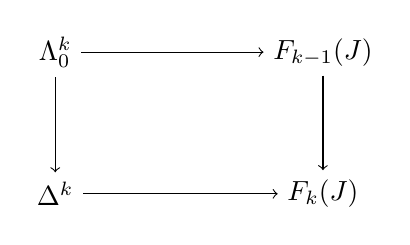
\begin{tikzpicture}
  \node (lk) at (0,0) {$\Lambda^k_0$};
  \node (rk) at (3.4,0) {$F_{k-1}(J)$};
  \node (ld) at (0,-1.8) {$\Delta^k$};
  \node (rd) at (3.4,-1.8) {$F_k(J)$};
  \draw[->] (lk) -- (rk);
  \draw[->] (lk) -- (ld);
  \draw[->] (ld) -- (rd);
  \draw[->] (rk) -- (rd);
\end{tikzpicture}
\end{center}
为了证明这一点，我们观察到：显然 $v_k \cup F_{k-1}(J)$ 的像等于 $F_k(J)$，于是只需看出
二者的交由 $\Lambda^k_0$ 给出。为此，我们考虑复合
$\Delta^{[k]\setminus\{i\}} \to \Delta^k \to F_k(J)$。对 $i = 0$，它由 $k-1$ 个可复合映射的
序列
\[
1 \to 0 \to 1 \to \dotsb,
\]
给出，该序列不包含于 $F_{k-1}(J)$ 之中。然而，若 $i \neq 0$，则它由一个以 $0$ 开头、
长度为 $k-1$ 的序列给出，从而由定义包含于 $F_{k-1}(J)$ 之中。

我们想证明映射
\[
\mathrm{Fun}(J, \D) \longrightarrow \mathrm{Fun}^{\simeq}(\Delta^1, \D)
\]
是一个\trJoyalEquivalence{}。这个映射有如下分解：
\[
\mathrm{Fun}(J, \D) \to \mathrm{Fun}^{\Delta^1}(F_k(J), \D) \to
\mathrm{Fun}^{\Delta^1}(F_{k-1}(J), \D) \to \mathrm{Fun}^{\simeq}(\Delta^1, \D).
\]
我们将证明中间的映射对所有 $k \ge 2$ 都是\trTrivialFibration{}。于是可得，映射
\[
\mathrm{Fun}(J, \D) \cong \lim_k \mathrm{Fun}^{\Delta^1}(F_k(J), \D)
\longrightarrow \mathrm{Fun}^{\simeq}(\Delta^1, \D)
\]
也是一个\trTrivialFibration{}，从而是一个\trJoyalEquivalence{}。于是我们需要证明：
对每个交换图表
\begin{center}
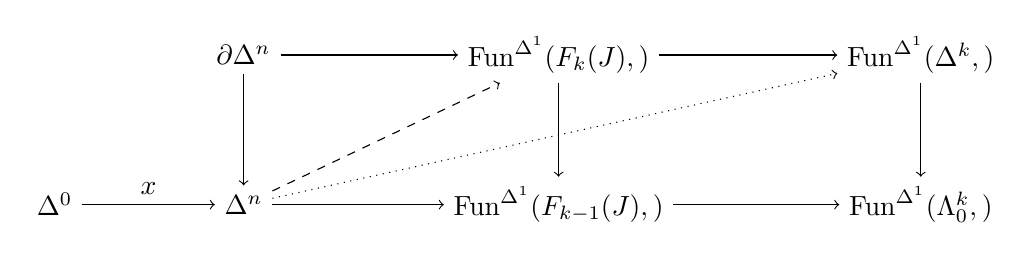
\begin{tikzpicture}
  \node (db) at (0,0) {$\partial \Delta^n$};
  \node (fk) at (4.0,0) {$\mathrm{Fun}^{\Delta^1}(F_k(J), \D)$};
  \node (dk) at (8.6,0) {$\mathrm{Fun}^{\Delta^1}(\Delta^k, \D)$};
  \node (d0) at (-2.4,-1.9) {$\Delta^0$};
  \node (dn) at (0,-1.9) {$\Delta^n$};
  \node (fkm) at (4.0,-1.9) {$\mathrm{Fun}^{\Delta^1}(F_{k-1}(J), \D)$};
  \node (lk) at (8.6,-1.9) {$\mathrm{Fun}^{\Delta^1}(\Lambda^k_0, \D)$};
  \draw[->] (db) -- (fk);
  \draw[->] (fk) -- (dk);
  \draw[->] (db) -- (dn);
  \draw[->] (d0) -- node[above] {$x$} (dn);
  \draw[->] (dn) -- (fkm);
  \draw[->] (fkm) -- (lk);
  \draw[->] (fk) -- (fkm);
  \draw[->] (dk) -- (lk);
  \draw[->, dashed] (dn) -- (fk);
  \draw[->, dotted] (dn) -- (dk);
\end{tikzpicture}
\end{center}
都存在一条使一切交换的虚箭头。我们断言，只需找到一条点箭头即可：显然，若去掉上标
$\Delta^1$，右边的方形便是一个\trPullback{}，此时这个\trPullback{}由所有这样的%
\trFunctor{} $F_k(J) \to \D$ 组成：其限制到 $\Delta^k$ 上把 $\Delta^1$ 送到一个%
\trEquivalence{}。这表明右边的方形是一个\trPullback{}。

经\trAdjunction{}，这个\trLiftingProblem{}对应于\trLiftingProblem{}%
\begin{center}
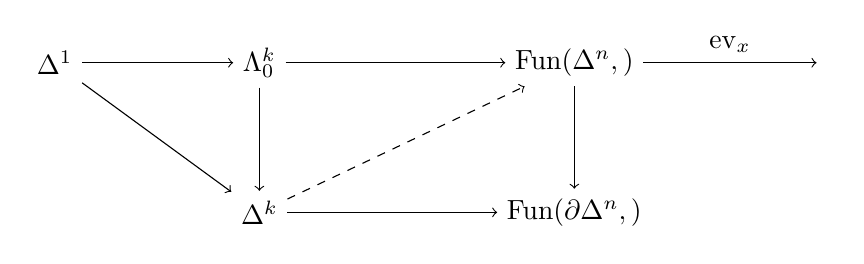
\begin{tikzpicture}
  \node (d1) at (0,0) {$\Delta^1$};
  \node (lk) at (2.6,0) {$\Lambda^k_0$};
  \node (fun) at (6.6,0) {$\mathrm{Fun}(\Delta^n, \D)$};
  \node (d) at (9.8,0) {$\D$};
  \node (dk) at (2.6,-1.9) {$\Delta^k$};
  \node (fb) at (6.6,-1.9) {$\mathrm{Fun}(\partial \Delta^n, \D)$};
  \draw[->] (d1) -- (lk);
  \draw[->] (lk) -- (fun);
  \draw[->] (fun) -- node[above] {$\mathrm{ev}_x$} (d);
  \draw[->] (d1) -- (dk);
  \draw[->] (lk) -- (dk);
  \draw[->] (dk) -- (fb);
  \draw[->] (fun) -- (fb);
  \draw[->, dashed] (dk) -- (fun);
\end{tikzpicture}
\end{center}
并且我们观察到，顶行的复合对 $\Delta^n$ 的每个\trObject{} $x$ 都是一个\trEquivalence{}。
因此，虚箭头由\trJoyal{}扩张定理给出，因为右边的竖直映射是一个\trInnerFibration{}，
而\trFunctor{} $\mathrm{Fun}(\Delta^n, \D) \to \prod_x \D$ 由\cref{thm:bijective-on-vertices}
是\trConservative{}。
\end{proof}

\begin{lemma}\label{lem:localization-all-morphisms}
对每个∞-\trCategory{} $\C$，沿 $\C$ 的全部\trMorphism{}的\trLocalization{}存在。
\end{lemma}

\begin{proof}
我们首先构造一个\trAnodyne{}映射 $f\colon \C \to X$，其靶为一个\trKanComplex{}%
（即∞-\trGroupoid{}）$X$：令 $Y$ 为\trPushout{}%
\begin{center}
\begin{tikzpicture}
  \node (tl) at (0,0) {$\coprod_{\alpha \in \C_1} \Delta^1$};
  \node (tr) at (3.6,0) {$\C$};
  \node (bl) at (0,-2.0) {$\coprod_{\alpha \in \C_1} J$};
  \node (br) at (3.6,-2.0) {$Y$};
  \draw[->] (tl) -- (tr);
  \draw[->] (tl) -- (bl);
  \draw[->] (tr) -- node[right] {$f$} (br);
  \draw[->] (bl) -- (br);
\end{tikzpicture}
\end{center}
\footnote{译注：按本句字面，$f$ 的靶为 $X$；但由下图（$f$ 标在 $\C \to Y$ 之箭上）
及后文「由于 $\Delta^1 \to J$ 是\trAnodyne{}的，故 $f$ 确实是\trAnodyne{}的」可知，
此处 $f$ 实指 $\C \to Y$，而到 $X$ 的\trAnodyne{}映射是其与 $g\colon Y \to X$ 的复合
$gf$。——译者注}由于 $\Delta^1 \to J$ 是\trAnodyne{}的（这由\cref{lem:delta1-j-localization} 的证明
得出），故 $f$ 确实是\trAnodyne{}的。随后，我们取一个内零调映射 $g\colon Y \to X$，其中 $X$
是一个∞-\trCategory{}：由\trSmallObjectArgument{}，我们可以把映射 $Y \to \ast$
分解为一个内零调映射随后接一个\trInnerFibration{}。由于 $g$ 是内零调的，复合 $gf$
是\trAnodyne{}的。我们断言，$X$ 其实是一个∞-\trGroupoid{}。为此，我们需要证明其%
\trHomotopyCategory{}是一个\trGroupoid{}。

由于映射 $Y \to X$ 是内零调的，它是一个\trJoyalEquivalence{}，从而在%
\trHomotopyCategory{}上诱导一个\trEquivalence{}。此外，取\trHomotopyCategory{}是%
\trNerve{}\trFunctor{}的\trLeftAdjoint{}，因而保持\trPushout{}，于是存在\trCategories{}的%
\trPushout{}%
\begin{center}
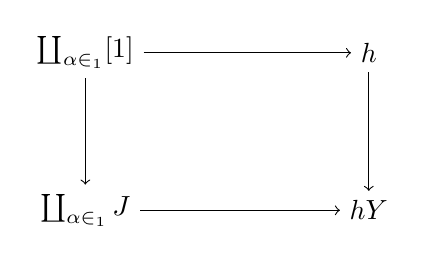
\begin{tikzpicture}
  \node (tl) at (0,0) {$\coprod_{\alpha \in \C_1} [1]$};
  \node (tr) at (3.6,0) {$h\C$};
  \node (bl) at (0,-2.0) {$\coprod_{\alpha \in \C_1} J$};
  \node (br) at (3.6,-2.0) {$hY$};
  \draw[->] (tl) -- (tr);
  \draw[->] (tl) -- (bl);
  \draw[->] (tr) -- (br);
  \draw[->] (bl) -- (br);
\end{tikzpicture}
\end{center}
因此，$hY$ 是由 $h\C$ 把 $\C$ 中全部\trMorphism{}逆转而得的（\cref{ex:pushout-groupoid}）。特别地，它是
一个\trGroupoid{}，从而 $hX$ 也是一个\trGroupoid{}。

最后，我们断言：对每个∞-\trCategory{} $\D$，限制\trFunctor{}%
$\mathrm{Fun}(X, \D) \to \mathrm{Fun}(\C, \D)$ 穿过一个\trTrivialFibration{}%
\[
\mathrm{Fun}(X, \D) \longrightarrow \mathrm{Fun}^{\simeq}(\C, \D).
\]
由于\trTrivialFibration{}由\cref{prop:trivial-kan-fibration-joyal-equivalence} 是%
\trJoyalEquivalence{}，故映射 $\C \to X$ 是一个\trLocalization{}。

显然，$\mathrm{Fun}(X, \D) \to \mathrm{Fun}(\C, \D)$ 穿过 $\mathrm{Fun}^{\simeq}(\C, \D)$，
因为 $X$ 是∞-\trGroupoid{}这一事实蕴含：$\C$ 中的每个\trMorphism{}都被映为 $X$ 中的
一个\trEquivalence{}。我们所关心的映射现在分解为
\[
\mathrm{Fun}(X, \D) \to \mathrm{Fun}(Y, \D) \to
\mathrm{Fun}^{\simeq}(\C, \D) \subseteq \mathrm{Fun}(\C, \D).
\]

第一个映射由\cref{thm:angle-fi-fibration} 第 (2) 部分是一个\trTrivialFibration{}，
因为 $g\colon Y \to X$ 是内零调的，而 $\D \to \ast$ 是一个\trInnerFibration{}。%
\footnote{译注：原书此处印作「since $Y \to X$ is an inner fibration」（因为
$Y \to X$ 是\trInnerFibration{}），但依本证明，$Y \to X$（即上述 $g$）是内零调映射；
\cref{thm:angle-fi-fibration} 第 (2) 部分在此所需的\trInnerFibration{}应是
$\D \to \ast$（由 $\D$ 是∞-\trCategory{}即得），兹径改。——译者注}第二个映射
位于下述图表之中
\begin{center}
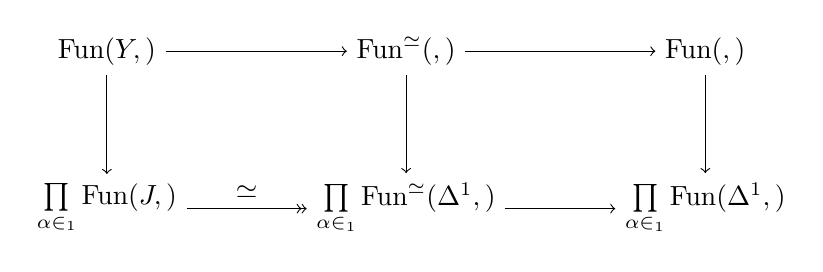
\begin{tikzpicture}
  \node (tl) at (0,0) {$\mathrm{Fun}(Y, \D)$};
  \node (tm) at (3.8,0) {$\mathrm{Fun}^{\simeq}(\C, \D)$};
  \node (tr) at (7.6,0) {$\mathrm{Fun}(\C, \D)$};
  \node (bl) at (0,-2.0) {$\prod\limits_{\alpha \in \C_1} \mathrm{Fun}(J, \D)$};
  \node (bm) at (3.8,-2.0)
    {$\prod\limits_{\alpha \in \C_1} \mathrm{Fun}^{\simeq}(\Delta^1, \D)$};
  \node (br) at (7.6,-2.0) {$\prod\limits_{\alpha \in \C_1} \mathrm{Fun}(\Delta^1, \D)$};
  \draw[->] (tl) -- (tm);
  \draw[->] (tm) -- (tr);
  \draw[->] (tl) -- (bl);
  \draw[->] (tm) -- (bm);
  \draw[->] (tr) -- (br);
  \draw[->>] (bl) -- node[above] {$\simeq$} (bm);
  \draw[->] (bm) -- (br);
\end{tikzpicture}
\end{center}
\footnote{译注：原书此图底行前两个 $\mathrm{Fun}$ 的靶印作 $\C$（即
$\prod_{\alpha \in \C_1}\mathrm{Fun}(J,\C)$ 与
$\prod_{\alpha \in \C_1}\mathrm{Fun}^{\simeq}(\Delta^1,\C)$），但依本证明——
大方形须由 $Y$ 的\trPushout{}定义为\trPullback{}，且左下方的水平映射须由%
\cref{lem:delta1-j-localization} 是\trTrivialFibration{}（其证明对每个靶∞-\trCategory{}%
均给出\trTrivialFibration{}）——底行诸靶均应为 $\D$，兹径改。——译者注}其中大方形由 $Y$ 的
定义是一个\trPullback{}，而右边的方形经细察是一个\trPullback{}。于是，左边的方形
也是一个\trPullback{}。由\cref{lem:delta1-j-localization}，左下方的水平映射是一个%
\trTrivialFibration{}，从而上方的水平映射亦然。这就完成了本引理的证明。
\end{proof}

\begin{remark}\label{rem:localization-left-adjoint}
我们稍后会看到，把 $\C$ 送到沿全部\trMorphism{}的\trLocalization{}这一对应，是
∞-\trGroupoid{}到∞-\trCategories{}之包含（作为∞-\trCategories{}之间的
∞-\trFunctor{}）的\trLeftAdjoint{}，见命题 5.1.12。
\end{remark}

\begin{proposition}\label{prop:localization-along-s}
对每个 $S \subseteq \C_1$，$\C$ 沿 $S$ 的\trLocalization{}存在。
\end{proposition}

\begin{proof}
对每个子集 $S \subseteq \C_1$，存在 $\C$ 的一个包含 $S$ 的最小子\trCategory{}%
$\C_S$：这对\trCategories{}是显然的，而对我们情形的陈述则通过对 $\C$ 的%
\trHomotopyCategory{}中相应的子\trCategory{}取\trPullback{}而得出。由此容易得出：$\C$ 沿 $\C_S$
的一个\trLocalization{}是 $\C$ 沿 $S$ 的一个\trLocalization{}，另见\cref{ex:iterated-localization}。

于是我们取 $\C_S$ 沿全部\trMorphism{}的一个\trLocalization{}，更精确地说，即如%
\cref{lem:localization-all-morphisms} 中那般的、到∞-\trGroupoid{} $X$ 的一个内零调
映射 $\C_S \to X$。然后我们考虑\trPushout{}%
\begin{center}
\begin{tikzpicture}
  \node (tl) at (0,0) {$\C_S$};
  \node (tr) at (2.8,0) {$\C$};
  \node (bl) at (0,-1.9) {$X$};
  \node (br) at (2.8,-1.9) {$W$};
  \draw[->] (tl) -- (tr);
  \draw[->] (tl) -- (bl);
  \draw[->] (tr) -- (br);
  \draw[->] (bl) -- (br);
\end{tikzpicture}
\end{center}
以及一个内零调映射 $g\colon W \to \D$，其中 $\D$ 是一个∞-\trCategory{}。然后，对一个
辅助∞-\trCategory{} $\E$，我们考虑图表
\begin{center}
\begin{tikzpicture}
  \node (tl) at (0,0) {$\mathrm{Fun}(\D, \E)$};
  \node (tm) at (3.9,0) {$\mathrm{Fun}(W, \E)$};
  \node (tr) at (7.4,0) {$\mathrm{Fun}^S(\C, \E)$};
  \node (bl) at (3.9,-1.9) {$\mathrm{Fun}(X, \E)$};
  \node (br) at (7.4,-1.9) {$\mathrm{Fun}^S(\C_S, \E)$};
  \draw[->] (tl) -- node[above] {$g^*$} (tm);
  \draw[->] (tm) -- (tr);
  \draw[->] (tm) -- (bl);
  \draw[->] (tr) -- (br);
  \draw[->] (bl) -- (br);
\end{tikzpicture}
\end{center}
并且我们断言右边的方形是一个\trPullback{}图表：为此，只需观察到每个\trFunctor{}%
$W \to \E$ 都把 $S$ 的像中的\trMorphism{}送到\trEquivalence{}，而这由它们在
$X$ 中被送到\trEquivalence{}这一事实得出。此外，下方的水平映射由前一步是一个%
\trTrivialFibration{}，从而上方的水平映射也是一个\trTrivialFibration{}。映射 $g^*$
是一个\trTrivialFibration{}，因为 $W \to \D$ 是内零调的。因此，上方的复合是一个%
\trTrivialFibration{}，从而是一个\trJoyalEquivalence{}。这表明映射 $\C \to \D$ 是沿
$S$ 的一个\trLocalization{}。
\end{proof}

除了「普遍地使\trMorphism{}成为\trInvertible{}」这一做法产出许多有趣的∞-\trCategories{}例子
（即便我们出发时的\trCategory{}是一个\trOrdinaryCategory{}）之外，我们还将在%
\cref{lem:localization-factorization} 中用它来证明∞-\trCategories{}之间的%
\trFunctor{}的一个分解性质。

\begin{example*}
考虑∞-\trCategories{}的 $1$-\trCategory{} $\mathrm{Cat}^1_{\infty}$，即
$\mathrm{sSet}$ 的以∞-\trCategories{}为\trObject{}的满子范畴。回忆，∞-\trCategories{}的
∞-\trCategory{} $\mathrm{Cat}_\infty$ 由这个\trCategory{}的同伦凝聚\trNerve{}%
$\mathrm{N}(\mathrm{Cat}^1_{\infty})$ 给出，并带有由 $\mathrm{Fun}(\C, \D)^{\simeq}$
给出的典范 Kan 充实。$\mathrm{Cat}^1_{\infty}$ 的恒等典范地细化成%
\trSimplicialCategories{}之间的一个\trFunctor{}：其在定义域上带常值单纯充实，
而其靶上带典范的单纯充实。换言之，我们得到一个典范的∞-\trCategories{}之间的\trFunctor{}%
\[
\mathrm{Cat}^1_{\infty} \longrightarrow \mathrm{Cat}_{\infty}.
\]
这个\trFunctor{}把\trJoyalEquivalence{}送到\trEquivalence{}：按定义，一个%
\trJoyalEquivalence{}是∞-\trCategories{}之间的一个映射，它在∞-\trCategory{}%
$\mathrm{Cat}_\infty$ 中成为一个\trEquivalence{}，见\cref{def:joyal-equivalence}。
于是，这个\trFunctor{}诱导一个\trFunctor{}%
\[
\mathrm{Cat}^1_{\infty}[\mathrm{Joy}^{-1}] \longrightarrow \mathrm{Cat}_{\infty}
\]
其中 $\mathrm{Joy}$ 表示\trJoyalEquivalence{}的集合。
\end{example*}

\begin{example*}
同样地，存在一个典范\trFunctor{} $\mathrm{Kan} \to \widehat{\mathrm{Spc}}$，它把%
\trHomotopy{}等价送到 $\widehat{\mathrm{Spc}}$ 中的\trEquivalence{}。于是，存在一个
诱导的\trFunctor{}%
\[
\mathrm{Kan}[\mathrm{he}^{-1}] \longrightarrow \widehat{\mathrm{Spc}},
\]
其中 $\mathrm{he}$ 表示\trKanComplex{}之间\trHomotopy{}等价的（大）集合。
\end{example*}

\begin{lemma}\label{lem:inclusions-induce-equivalences}
包含 $\mathrm{Kan} \to \mathrm{sSet}$ 与 $\mathrm{Cat}^1_{\infty} \to \mathrm{sSet}$
诱导\trEquivalence{}%
\[
\mathrm{Kan}[\mathrm{he}^{-1}] \simeq \mathrm{sSet}[\mathrm{we}^{-1}]
\quad\text{以及}\quad
\mathrm{Cat}^1_{\infty}[\mathrm{Joy}^{-1}] \simeq \mathrm{sSet}[\mathrm{Joy}^{-1}].
\]
\end{lemma}

\begin{proof}
\trSmallObjectArgument{}提供了\trFunctor{}%
$F\colon \mathrm{sSet} \to \mathrm{Cat}^1_{\infty}$ 与
$G\colon \mathrm{sSet} \to \mathrm{Kan}$：把映射
$X \to \ast$ 函子式地分解为一个内零调映射随后接一个\trInnerFibration{}，相应地，
分解为一个\trAnodyne{}映射随后接一个\trKanFibration{}。我们断言，这两个\trFunctor{}%
分别把\trJoyalEquivalence{}送到\trJoyalEquivalence{}、把弱同伦等价送到弱同伦等价。
为了看到这一点，设 $X \to Y$ 是这样一个等价。于是我们有交换图表
\begin{center}
\begin{tikzpicture}
  \node (x) at (0,0) {$X$};
  \node (c) at (2.8,0) {$\C$};
  \node (y) at (0,-1.8) {$Y$};
  \node (d) at (2.8,-1.8) {$\D$};
  \draw[->] (x) -- (c);
  \draw[->] (y) -- (d);
  \draw[->] (x) -- (y);
  \draw[->] (c) -- (d);
\end{tikzpicture}
\end{center}
其中水平映射是内零调的，从而是\trJoyalEquivalence{}。由\trJoyalEquivalence{}的%
\trThreeForTwoProperty{}，我们发现：$\C \to \D$ 是一个\trJoyalEquivalence{}，当且仅当
$X \to Y$ 是一个\trJoyalEquivalence{}。对弱同伦等价的论证是一样的。于是，这个%
\trFunctor{}诱导一个\trFunctor{}%
\[
\mathrm{sSet}[\mathrm{Joy}^{-1}] \longrightarrow
\mathrm{Cat}^1_{\infty}[\mathrm{Joy}^{-1}],
\]
我们断言它是典范\trFunctor{}%
\[
\mathrm{Cat}^1_{\infty}[\mathrm{Joy}^{-1}] \longrightarrow
\mathrm{sSet}[\mathrm{Joy}^{-1}]
\]
（由包含所诱导）的一个逆。

为此，我们观察到映射 $X \to \C = F(X)$ 确定了一个从 $\mathrm{sSet}$ 的恒等到复合
$iF\colon \mathrm{sSet} \to \mathrm{sSet}$ 的\trNaturalTransformation{}。更精确地说，
它确定一个映射
\[
\Delta^1 \longrightarrow \mathrm{Fun}(\mathrm{sSet}, \mathrm{sSet})
\longrightarrow \mathrm{Fun}(\mathrm{sSet}, \mathrm{sSet}[\mathrm{Joy}^{-1}])
\]
我们断言它落入由那些把\trJoyalEquivalence{}送到\trEquivalence{}的\trFunctor{}组成的
满子范畴之中：这是因为 $F$（显然 $i$ 也一样）把\trJoyalEquivalence{}送到%
\trJoyalEquivalence{}，正如我们刚刚论证的那样。于是，由\trLocalization{}的%
\trUniversalProperty{}，
我们得到一个映射
\[
\Delta^1 \longrightarrow
\mathrm{Fun}(\mathrm{sSet}[\mathrm{Joy}^{-1}], \mathrm{sSet}[\mathrm{Joy}^{-1}])
\]
其在 $0$ 与 $1$ 上的限制分别由恒等与一个\trFunctor{}给出，而后者的限制到
$\mathrm{sSet}$ 上由复合 $iF$ 所诱导。对一个固定的\trObject{} $X \in \mathrm{sSet}$，
所得的\trMorphism{}由 $X \to F(X)$ 给出，而我们已论证过它是\trJoyalEquivalence{}。
特别地，上面给出的 $1$-\trSimplex{}是 $\mathrm{sSet}[\mathrm{Joy}^{-1}]$ 的恒等与由
$iF$ 所诱导的\trFunctor{}之间的一个\trNaturalEquivalence{}。\footnote{译注：原书此两处
均印作「the composite Fi」与「induced by Fi」，但依前文，此处的复合应为
$iF\colon \mathrm{sSet} \to \mathrm{sSet}$（$F$ 在前、包含 $i$ 在后），$Fi$
不合上下文，兹径改。——译者注}

尚需证明：由复合 $iF$ 所诱导的\trFunctor{}也是一个\trEquivalence{}。为此，我们用类似的论证发现：
映射 $X \to FX$ 诱导一个逐点为\trJoyalEquivalence{}的变换 $\mathrm{id} \to iF$。这就
证明了本引理关于\trJoyalEquivalence{}的部分，而对弱同伦等价的论证是一样的。
\end{proof}

下述定理非常重要，但超出了本书的范围。一个类似的结果对单纯\trModelCategory{}一般地成立，
见 \cite[Theorem 1.3.4.20]{Lur17}。我们稍后将讨论这个结果之证明的若干步骤，
见推论 3.2.26。

\begin{theorem}\label{thm:localization-canonical-equivalences}
典范\trFunctor{} $\mathrm{sSet}[\mathrm{we}^{-1}] \to \mathrm{Spc}$ 与
$\mathrm{sSet}[\mathrm{Joy}^{-1}] \to \mathrm{Cat}_\infty$ 是∞-\trCategories{}之间的%
\trEquivalence{}。
\end{theorem}

我们以一个有用的分解构造来结束本节。

\begin{definition}\label{def:path-fibration}
设 $f\colon \C \to \D$ 是∞-\trCategories{}之间的一个\trFunctor{}。我们用单纯集的如下%
\trPullback{}来定义 $f$ 的\emph{\trPathFibration{}}（path-fibration）$P(f)$：
\begin{center}
\begin{tikzpicture}
  \node (tl) at (0,0) {$P(f)$};
  \node (tr) at (3.6,0) {$\mathrm{Fun}(J, \D)$};
  \node (bl) at (0,-1.9) {$\C$};
  \node (br) at (3.6,-1.9) {$\D$};
  \draw[->] (tl) -- (tr);
  \draw[->] (tl) -- (bl);
  \draw[->] (tr) -- node[right] {$s$} (br);
  \draw[->] (bl) -- node[above] {$f$} (br);
\end{tikzpicture}
\end{center}
其中 $s$ 是源映射。
\end{definition}

考虑映射 $\C \to \mathrm{Fun}(J, \D)$，它伴随于复合映射 $\C \times J \to \C \to \D$。
它把一个\trObject{} $x$ 送到 $f(x)$ 的恒等\trMorphism{}。显然，这个\trFunctor{}与 $s$
的复合由 $f$ 给出，因此我们得到一个诱导映射 $c\colon \C \to P(f)$，它是典范映射
$P(f) \to \C$ 的一个\trSectionMap{}。特别地，$c$ 是一个\trMonomorphism{}。此外，
$P(f) \to \mathrm{Fun}(J, \D)$ 与目标映射 $\mathrm{Fun}(J, \D) \to \D$ 的复合给出复合
\[
\C \xrightarrow{c} P(f) \xrightarrow{t} \D.
\]
这个复合由 $f$ 给出，于是我们得到了 $f$ 穿过 $P(f)$ 的一个分解。

\begin{lemma}\label{lem:localization-factorization}
设 $f\colon \C \to \D$ 是∞-\trCategories{}之间的一个\trFunctor{}，并设
$\C \xrightarrow{c} P(f) \xrightarrow{t} \D$ 是我们刚刚构造的分解。那么，$c$ 是一个%
\trJoyalEquivalence{}，而 $t$ 是一个\trIsofibration{}。特别地，∞-\trCategories{}之间
的任何映射 $f\colon \C \to \D$ 都能分解为一个作为\trMonomorphism{}的%
\trJoyalEquivalence{}，随后接一个\trIsofibration{}。
\end{lemma}

\begin{proof}
我们断言：源映射 $s\colon \mathrm{Fun}(J, \D) \to \D$ 是一个\trTrivialFibration{}。
由\cref{lem:trivial-fibration-joyal-isofibration}，只需证明它既是一个%
\trJoyalEquivalence{}又是一个\trIsofibration{}。有许多论证可以表明
$\Delta^0 \to J$ 是一个\trJoyalEquivalence{}（例如，二者都是\trOrdinaryCategory{}，
而该\trFunctor{}显然是\trOrdinaryCategory{}之间的一个\trEquivalence{}），于是由%
\cref{prop:joyal-equivalence-precomposition} 可得，诱导映射
$\mathrm{Fun}(J, \D) \to \mathrm{Fun}(\Delta^0, \D) \cong \D$ 也是一个%
\trJoyalEquivalence{}。由\cref{prop:isofibration-induced-functor}，沿一个映入
∞-\trCategory{}的\trMonomorphism{}取限制是一个\trIsofibration{}，于是我们得出结论：
$\mathrm{Fun}(J, \D) \to \D$ 是一个\trTrivialFibration{}，如所断言。于是，作为这个
映射的一个\trPullback{}，\trFunctor{} $P(f) \to \C$ 也是一个\trTrivialFibration{}。
由于复合
\[
\C \to P(f) \to \C
\]
是恒等（由构造可知），由\trJoyalEquivalence{}的\trThreeForTwoProperty{}可得：映射
$\C \to P(f)$ 如所断言是一个\trJoyalEquivalence{}。

为了看出 $P(f) \to \D$ 是一个\trIsofibration{}，我们观察到方形
\begin{center}
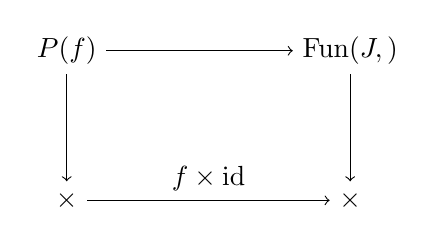
\begin{tikzpicture}
  \node (tl) at (0,0) {$P(f)$};
  \node (tr) at (3.6,0) {$\mathrm{Fun}(J, \D)$};
  \node (bl) at (0,-1.9) {$\C \times \D$};
  \node (br) at (3.6,-1.9) {$\D \times \D$};
  \draw[->] (tl) -- (tr);
  \draw[->] (tl) -- (bl);
  \draw[->] (tr) -- (br);
  \draw[->] (bl) -- node[above] {$f \times \mathrm{id}$} (br);
\end{tikzpicture}
\end{center}
也是一个\trPullback{}，并且再次由\cref{prop:isofibration-induced-functor}，右边的
竖直映射是一个\trIsofibration{}。于是，$P(f) \to \C \times \D$ 也是一个%
\trIsofibration{}，见\cref{cor:isofibration-stable-pullback}。由于投射
$\C \times \D \to \D$ 也是一个\trIsofibration{}，本引理得证。
\end{proof}
